%%%%%%%%%%%%%%%%%%%%%%%%%%%%%%%%%%%%%%%%%%%%%%%%%%%%%%%%%%%%%%%%%%%%%%%%%%%%%%%%
% \section{Numerical Results}
%%%%%%%%%%%%%%%%%%%%%%%%%%%%%%%%%%%%%%%%%%%%%%%%%%%%%%%%%%%%%%%%%%%%%%%%%%%%%%%%

\begin{figure}
\begin{center}
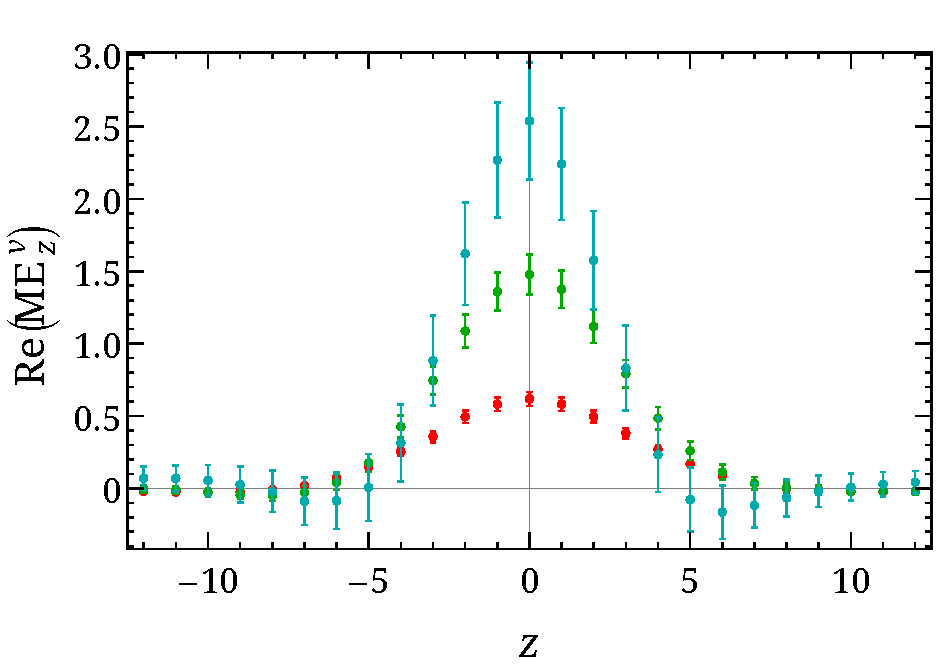
\includegraphics[width=0.48\textwidth]{images/parton-re-MEzv-vs-z_two-two} 
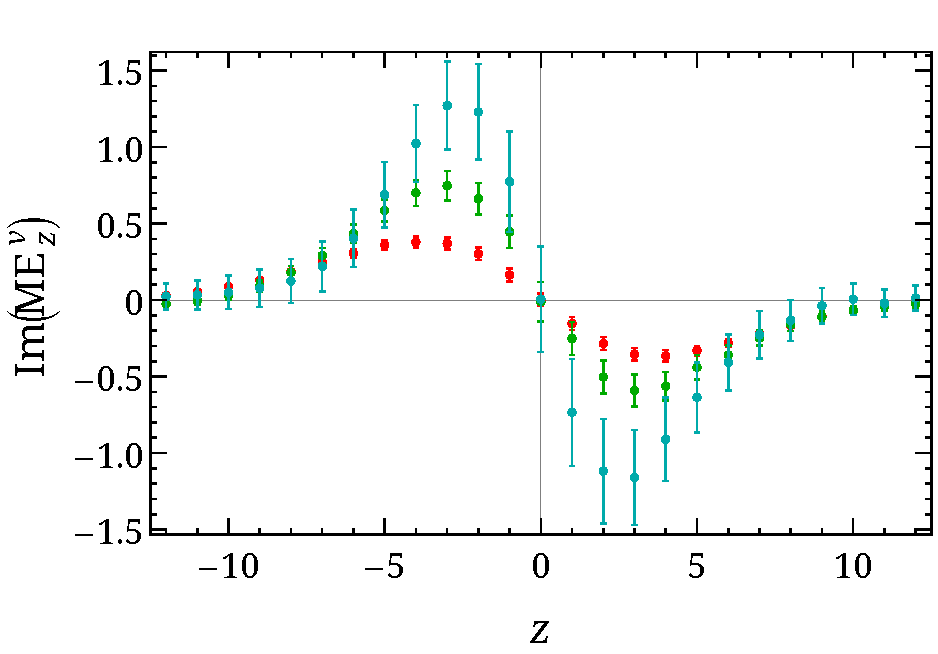
\includegraphics[width=0.48\textwidth]{images/parton-im-MEzv-vs-z_two-two}
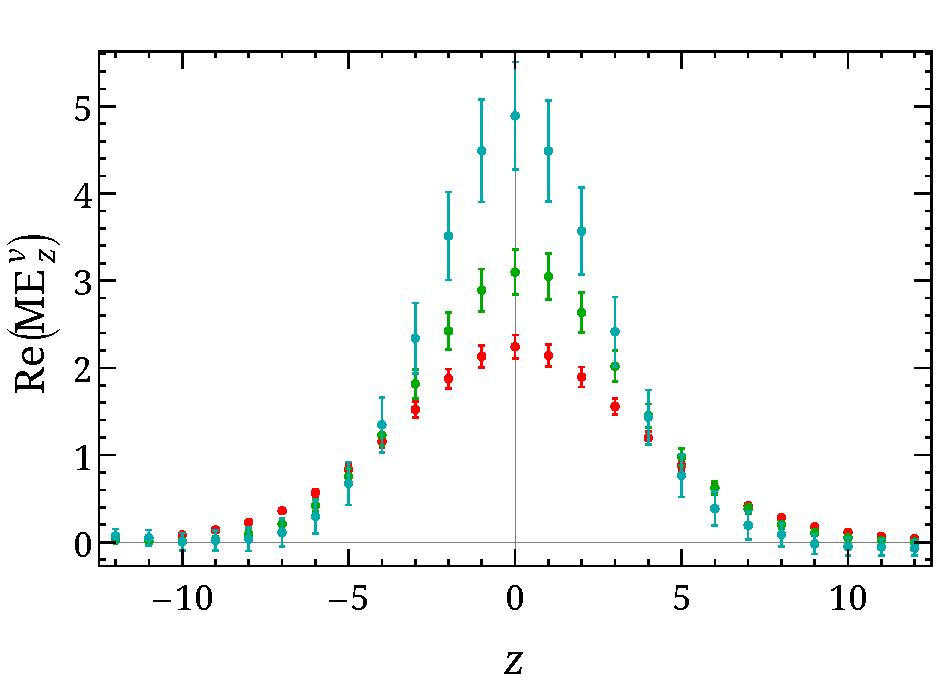
\includegraphics[width=0.48\textwidth]{images/helicity-re-MEzv-vs-z_two-two} 
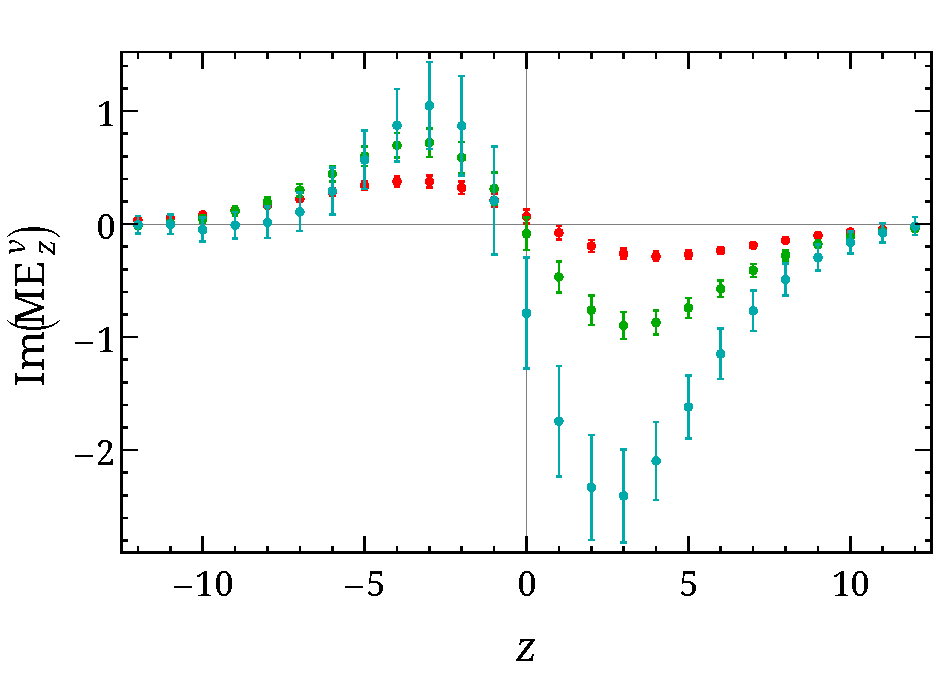
\includegraphics[width=0.48\textwidth]{images/helicity-im-MEzv-vs-z_two-two}
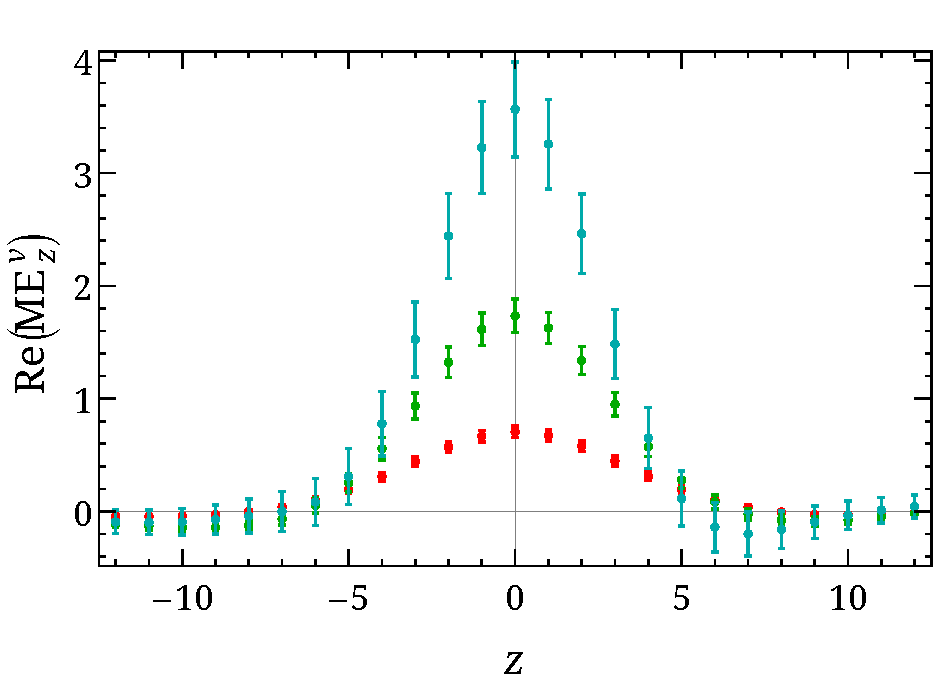
\includegraphics[width=0.48\textwidth]{images/transversity-re-MEzv-vs-z_two-two} 
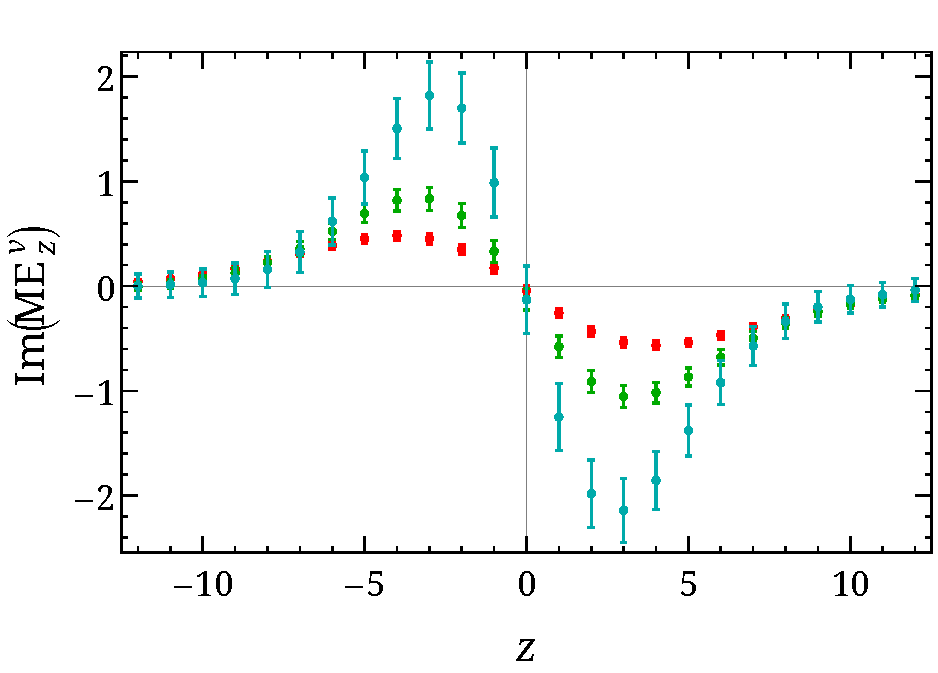
\includegraphics[width=0.48\textwidth]{images/transversity-im-MEzv-vs-z_two-two}
\end{center}
\caption{The real (left) and imaginary (right) parts of the nonlocal isovector matrix elements (defined in Eq.~\ref{eq:qlat}) needed to determine the quark density (top), helicity (middle) and transverse (bottom) PDFs as functions of the length $z$ of the gauge connection between the quark and antiquark fields in the current insertion. The different colors from bottom to top indicate 
boosted momentum $P_z$ (in units of $2\pi/L$) of 1 (red), 2 (green), 3 (cyan)
.}
\label{fig:ME}
\end{figure}

In this paper, we report the results of a lattice-QCD calculation using clover valence fermions on an ensemble of gauge configurations with lattice spacing $a=0.12$~fm, box size $L\approx 3$~fm and pion mass $M_\pi \approx 310$~MeV with $N_f=2+1+1$ (degenerate up/down, strange and charm) flavors of highly improved staggered quarks (HISQ)~\cite{Follana:2006rc} generated by MILC Collaboration~\cite{Bazavov:2012xda}. The gauge links are hypercubic (HYP)-smeared~\cite{Hasenfratz:2001hp} and then clover parameters are tuned to recover the lowest pion mass of the staggered quarks in the sea\footnote{This setup is the same as the one used in works done by PNDME~\cite{Bhattacharya:2015wna,Bhattacharya:2015esa,Bhattacharya:2013ehc}.}.
HYP smearing has been shown to significantly improve the discretization effects on operators and shift their corresponding renormalizations toward their tree-level values (near 1 for quark bilinear operators). 
The volume of this ensemble is large enough, $M_\pi L \approx 4.5$, that there is no visible finite-volume correction in current lattice-QCD calculations of nucleon matrix elements. 
The results shown in this work are done using correlators calculated from 3 source locations on 449 configurations.

%%%%%%%%%%%%%%%%%%%%%%%%%%%%%%%%%%%%%%%%
% Nucleon Matrix Elements 
On the lattice, we first calculate the time-independent, nonlocal (in space, chosen to be the $z$ direction) correlators of a nucleon with finite-$P_z$ boost
%
\begin{align}
\label{eq:qlat}
\tilde{h}_\text{lat}(z,\mu,P_z) =  
  \left\langle \vec{P} \right|
    \bar{\psi}(z) \Gamma \left( \prod_n U_z(n\hat{z})\right) \psi(0)
  \left| \vec{P} \right\rangle,
\end{align}
%
where $U_z$ is a discrete gauge link in the $z$ direction and $\vec{P}=\{0,0,P_z\}$ is the momentum of the nucleon. $\Gamma=\gamma_z$, $\gamma_z\gamma_5$ and $\sigma_{xz}\gamma_5$ for the unpolarized, helicity, and transversity distributions, respectively. The spin direction is along the $z$-direction for helicity and  $x$-direction for transversity.
In this work, we are only studying 
isovector quantities (such as the up-down flavor asymmetry).
To control the systematics due to contamination by nearby excited-state quantities, 
we make a simultaneous fit of the nucleon matrix element correlators,
using two source-sink nucleon separations, 0.96 and 1.2~fm; 
the detailed procedure is described in Ref.~\cite{Bhattacharya:2013ehc} for the nucleon charges.
Examining the individual fits to each source-sink nucleon separation, we do not see noticeable excited-state contamination for either 
separation at the current statistics. 
Figure~\ref{fig:ME} shows the bare lattice nucleon matrix elements at the three boost momenta used here: $\{1,2,3\} 2\pi/L$, which correspond to nucleon momenta of 0.43, 0.86 and 1.29~GeV, respectively. 
We note that in all three cases, the matrix elements vanish when the link length reaches 10--12.
The signal-to-noise ratios worsen as the nucleon is increasingly boosted, so to push this method forward, future studies should investigate methods for improving nucleon momentum sources.

%%%%%%%%%%%%%%%%%%%%%%%%%%%%%%%%%%%%%%%%
% Quasi-distributions
We then take the integrals to transform the lattice matrix elements as functions of spatial link length $z$ into the quasi-distributions as functions of parton momentum fraction $x$:
%
\begin{align}
\label{eq:qlat}
\tilde{q}(x,\Lambda,P_z) = \int \frac{dz}{4\pi} e^{-i z k} C_\Gamma \tilde{h}_\text{lat}(z,\Lambda,P_z),
\end{align}
% 
where $x=k/P_z$, $\Lambda$ is the renormalization scale set by the lattice spacing $a$ and $C_\Gamma=(P_z/M S_z)$ for helicity and $C_\Gamma=1$
for unpolarized and transversity PDFs.
%Note that $k$ is an arbitrary constant in the integral; w
We have sampled $\delta k$ as finely as 0.002 but have
not observed any dependence in downstream results on the choice of interval used here.
Since the matrix elements go to zero beyond about 12, the integral does not depend sensitively on the 
choice of maximum $z$. % in the range from 10 to 15.
The normalization of the long-link operators is currently 
estimated through zeroth moment of the quark distribution,
%
\begin{equation}
\label{eq:49}
\tilde{q}(x,\mu,P_z) \rightarrow \frac{\tilde{q}(x,\mu,P_z)}{\int\!dx\,\tilde{q}(x,\mu,P_z)} \times
  g_V^\text{local}(\mu=2\mbox{ GeV})_{\overline{\text{MS}}}.
\end{equation}
%
This choice reduces the systematic uncertainty arising from the matching
and other systematics such as finite-volume effects and lattice discretization. 
Given that the lattice renormalization constants for most observables are close to 1 on this ensemble,
we will get reasonable cancellation of the remaining factors. 
Similar normalizations apply to the helicity and transversity. 
The normalization of each distribution is then set by multiplying in
the corresponding vector, axial or tensor charge, as obtained on the
same lattices by Ref.~\cite{Bhattacharya:2013ehc} using standard techniques.

The isovector nucleon quark, helicity and transversity quasi-distributions are shown in 
Fig.~\ref{fig:intx}, using in the same color scheme to indicate different boosted momenta.
We see that our lattice-QCD result has nonzero values for $q(x)$, $\Delta q(x)$ and $\delta q(x)$ at $x \ge 1$ and that it does not vanish until $x \approx 1.5$. %
%
In all three cases, the smallest momentum has the widest distribution, spreading out to 
large positive and negative $x$, beyond $|x|=1$. 
As we discussed after Eq.~\ref{q}, when $P_z$ is finite, the range of $|x|$ is not bounded by unity.
But as the boosted momentum increases, the distribution sharpens
and narrows, decreasing the contribution coming from the $|x|>1$ regions, just what we would expect 
in the lightcone distribution.
% 
This is not hard to understand (as we discussed in our earlier work~\cite{Lin:2014zya}): in the infinite-momentum frame, no constituents of the nucleon can carry more momentum than the nucleon as a whole. However, since the momentum in our calculation is finite, the PDF does not have to vanish at $x=1$. 
%
The peak location for the
density and helicity distributions remains roughly the same for $P_z=$ 2 and 3, but in the case of the
transversity, the peak shifts toward $x=0$ for $P_z=3$.
Note that there is a substantial difference in magnitude between $P_z$ = 2 and 3, and an even more severe difference in shape between $P_z=1$ and the others. 
We note that since $x$ is defined as $k/P_z$ and $k$ is arbitrary, we can make $k$ as small as desired to obtain small-$x$ physics.
However, the small-$x$ region corresponds to long-distance physics, which requires longer physical links to probe. This is similar to the finite-volume effect commonly seen in LQCD calculations, except the large-$z$ links are essential to obtain a reasonable description of the physics in this region.

\begin{figure}
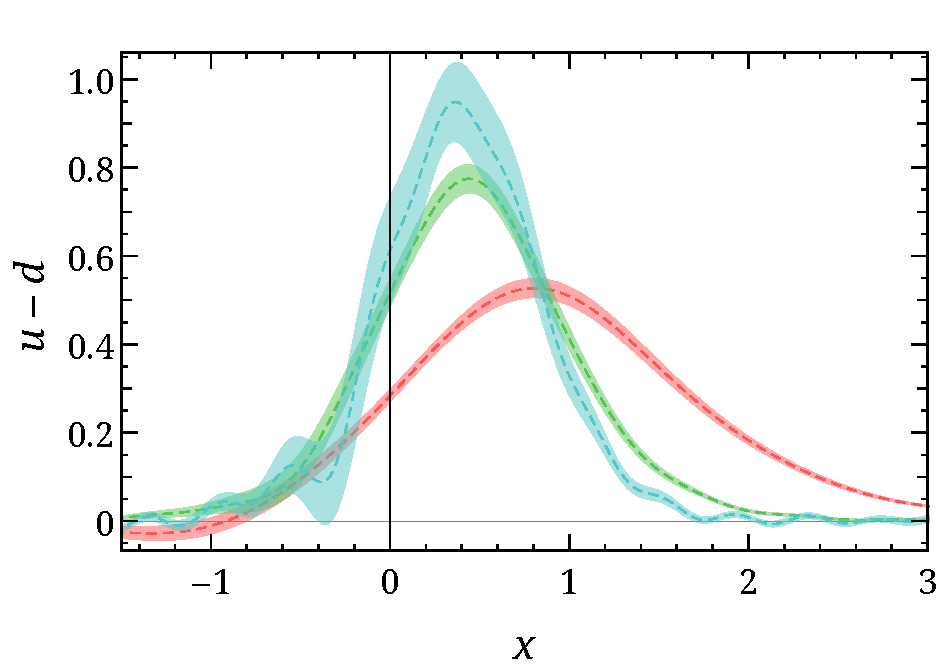
\includegraphics[width=0.32\textwidth]{images/parton-intv-vs-x_two-two}
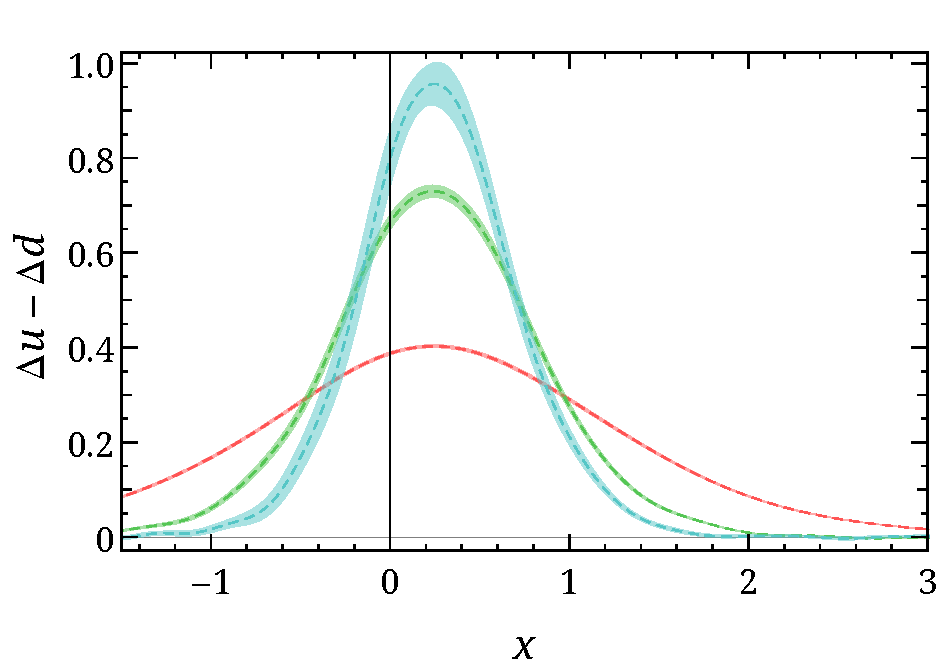
\includegraphics[width=0.32\textwidth]{images/helicity-intv-vs-x_two-two}
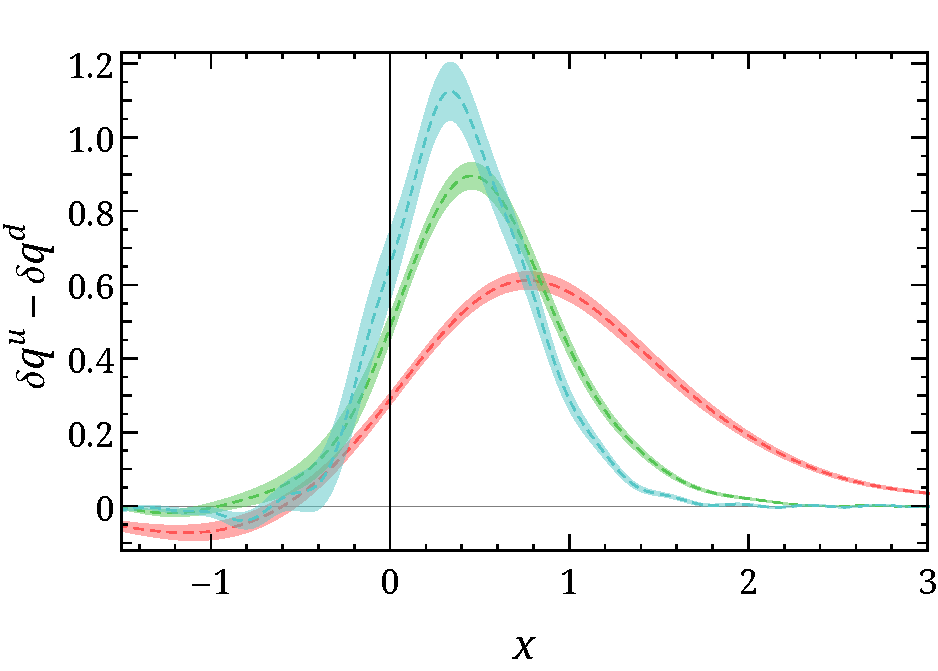
\includegraphics[width=0.32\textwidth]{images/transversity-intv-vs-x_two-two}
\caption{The nucleon isovector quasi-PDFs of Eq.~\ref{eq:49}
for the quark density (left), helicity (middle) and transversity (right) as functions of $x$. The different colors from $P_z$ (in units of $2\pi/L$) 1 (red), 2 (green), 3 (cyan).
We see the data converging at large $P_z$.}
\label{fig:intx}
\end{figure}

%%%%%%%%%%%%%%%%%%%%%%%%%%%%%%%%%%%%%%%%
% Corrections
To improve the quasi-distribution closer to the infinite-momentum frame (IMF) proton distribution functions, we follow the recipes described in
Sec.~\ref{sec:corrections} for the one-loop and mass corrections. 
The effects of the one-loop (with $\alpha_s$ set to 0.2) and the final quark distribution (one-loop first, 
followed by mass correction) and original quasi-distribution are shown in Fig.~\ref{fig:corrections} for $P_z=2$ and $P_z=3$. We found that corrections for $P_z=1$ distributions are poorly behaved due to the smallness of the boosted momentum; the results are ignored here. 
First, we compare the quasi- (green band) and one-loop--corrected (red band) distributions. 
For quark density, helicity and transversity distributions, 
we find a significant dip caused by the one-loop correction near $x=0$.
The depth of this dip 
increases as we increase the resolution in $x$, $dx$, used in the integral; 
this artifact may disappear with proper one-loop renormalization in the future calculations.
We also observe a clear evidence of higher values of the peak in the positive-$x$ area and pushing outward of the peak location of the distribution. In the large-$x$ region, the distribution is pulling back, making it rarer for quarks to carry a large
fraction of momentum as one approaches the IMF, which is what we expect. 
For the $P_z=3$ distribution, the magnitude of the changes due to the one-loop correction decrease, as expected.
As we expand the reach of the lattice calculation to larger values of $P_z$, the corrections will be even smaller. 
The pushing outward in the large-$x$ region
may be caused
by the validity of the one-loop correction requiring larger momentum. Future calculations should be
designed to study this further with larger momentum and higher statistics. 

We then apply the mass-correction formula to the one-loop--corrected distribution, shown as blue bands in 
Fig.~\ref{fig:corrections} for all distributions and both $P_z\in\{2,3\}$. 
The peaks are shifted toward $x=0$, the distribution sharpens, and the large-$x$ region distribution is suppressed further, as expected. 
In both the quark density and transversity distributions,
the mass correction also reduces the depth of the dip caused by the one-loop correction formula, 
and the effect of the mass correction also diminishes for the $P_z=3$ case. 
However, for the helicity, the mass-correction
causes a significant unphysical spike rising near $x=0$ due to the singularity in the double-integral terms. 
We note that the peak significantly decreases between $P_z=2$ and $P_z=3$,
and this should be reduced with larger $P_z$ data in the future. 
The height of the peak depends on the resolution of the integral, but has very small effect on the zeroth moment.  
In addition, the mass-correction formulae used in this paper differ from
what we used in our earlier publication, Ref.~\cite{Lin:2014zya}.
This change shifts the central value of the unpolarized and longitudinally polarized up-down quark
asymmetry and increases the estimated errors. However, the results remain consistent within the given errors.

To further reduce the remaining
$\mathcal{O}(\Lambda_\text{QCD}^2/P_z^2)$ correction due to higher-twist operators, 
we extrapolate to infinite momentum using the form $a + b /P_z^2$ at each $x$ point.
The resulting distribution, shown in Fig.~\ref{fig:IpM-distribution}, has $|x| > 1$ region within 2 sigma of zero;
thus, we recover the correct support for the physical distribution within error.
Note that the smallest reliable region of $x$ is related to the largest
momentum on available on the lattice $\mathcal{O}(1/a)$, which is roughly the
inverse of length of the lattice volume in the link direction; therefore, 
we expect large systematic uncertainty in the region $x \in [-0.08,0.08]$.
In the case of quark density,
there are also indications of momentum convergence within 2 sigma from $P_z=2$ and 3 data. 
In addition, the final extrapolated distribution (orange band) is consistent with the largest momentum 
distribution. However, for the polarized distributions, even larger $P_z$ calculations are needed to improve the convergence rate and reduce the uncertainty due to extrapolation, especially for the helicity.
 
\begin{figure}
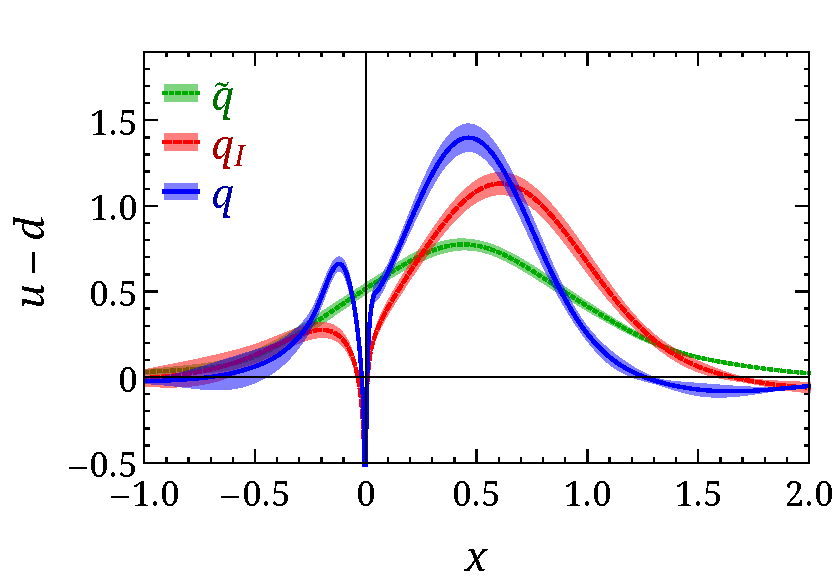
\includegraphics[width=0.32\textwidth]{images/evolution-comp-parton-p2-dx200.pdf}
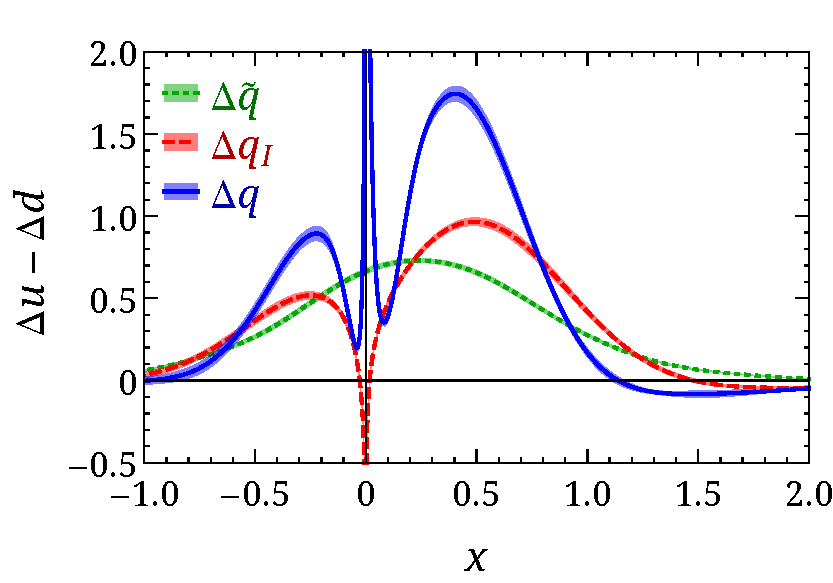
\includegraphics[width=0.32\textwidth]{images/evolution-comp-helicity-p2-dx200.pdf}
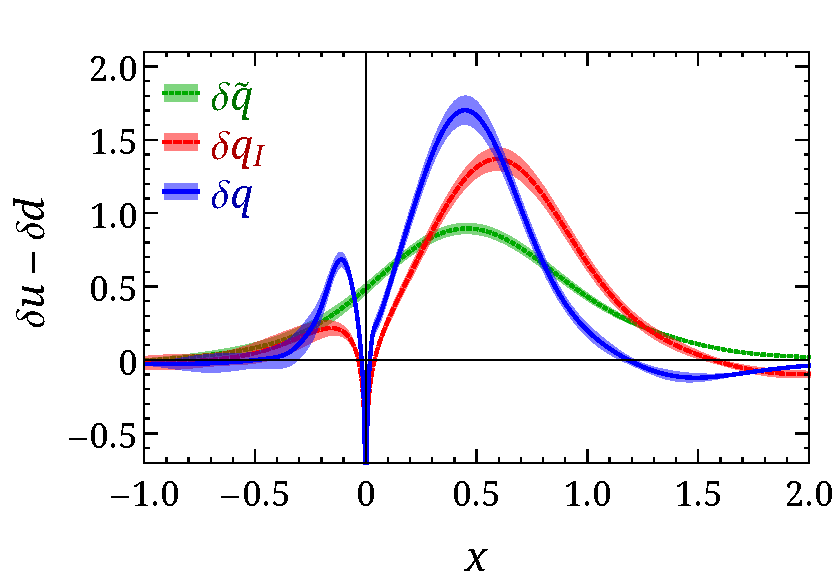
\includegraphics[width=0.32\textwidth]{images/evolution-comp-transversity-p2-dx200.pdf}

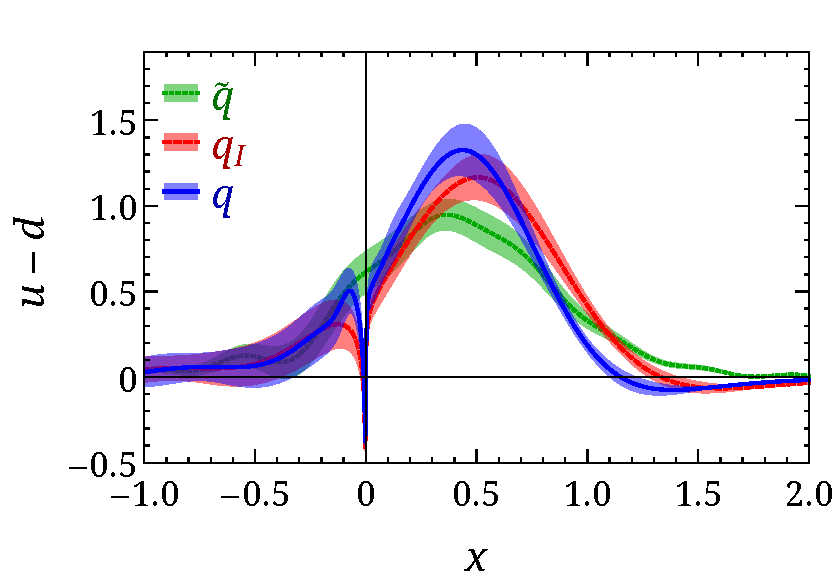
\includegraphics[width=0.32\textwidth]{images/evolution-comp-parton-p3-dx200.pdf}
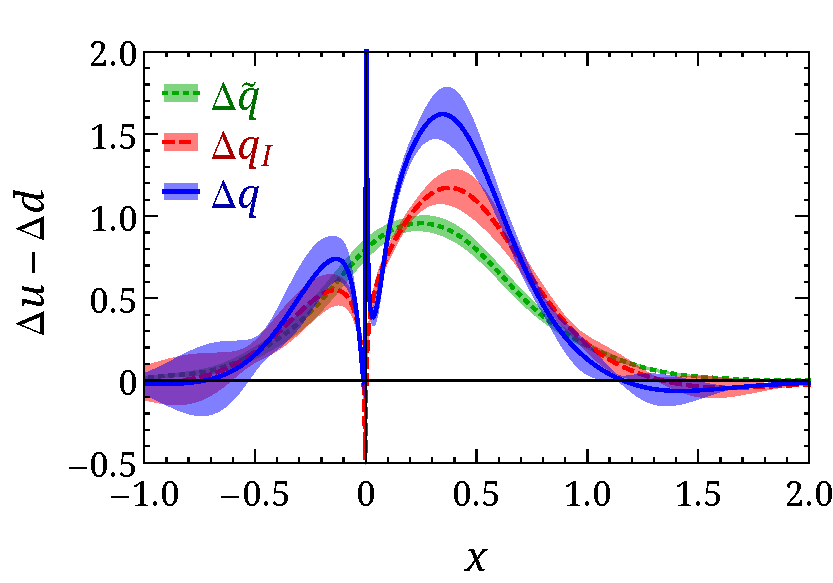
\includegraphics[width=0.32\textwidth]{images/evolution-comp-helicity-p3-dx200.pdf}
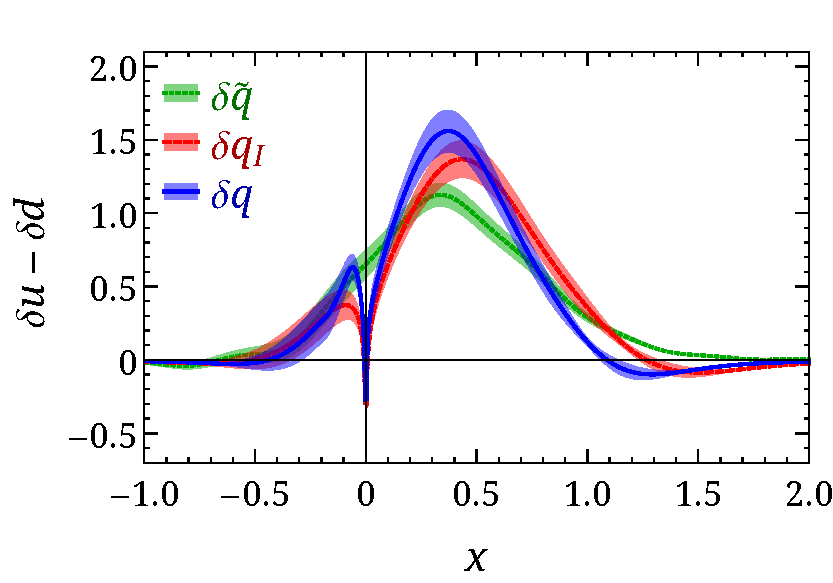
\includegraphics[width=0.32\textwidth]{images/evolution-comp-transversity-p3-dx200.pdf}

\caption{The nucleon isovector quasi-PDF (green), with one-loop correction (red), 
and with after one-loop and mass correction (i.e. $q_{II}$).
(blue) for the
 quark density (left), helicity (middle) and transversity (right) as functions of $x$ for the higher two boosted 
momenta $P_z = 2$ (top row) and $3$ (bottom row) in units of $2\pi/L$. 
}
\label{fig:corrections}
\end{figure}


\begin{figure}
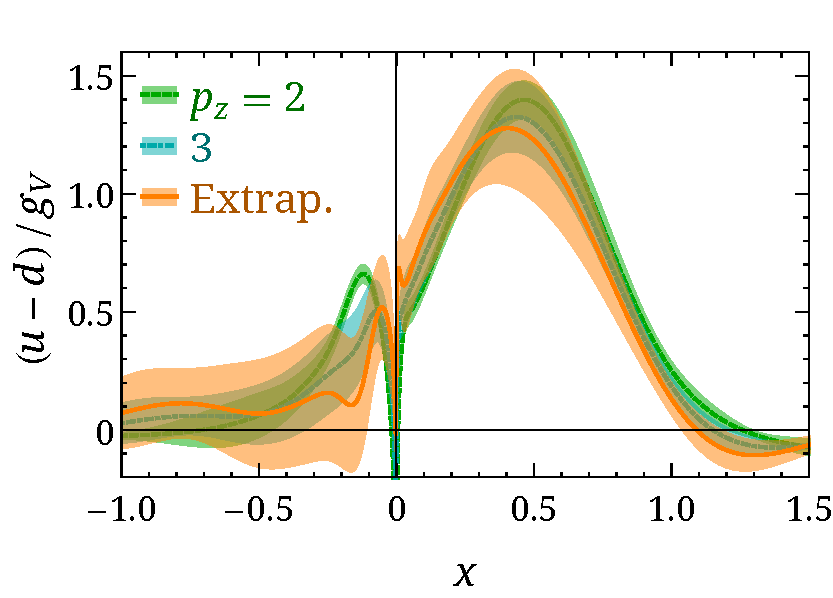
\includegraphics[width=0.32\textwidth]{images/loopscale-parton-new.pdf}
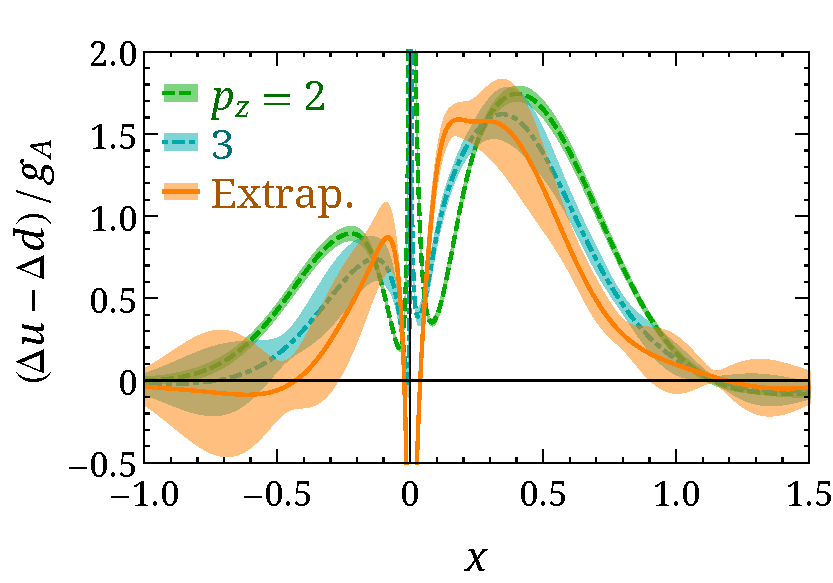
\includegraphics[width=0.32\textwidth]{images/loopscale-helicity-new.pdf}
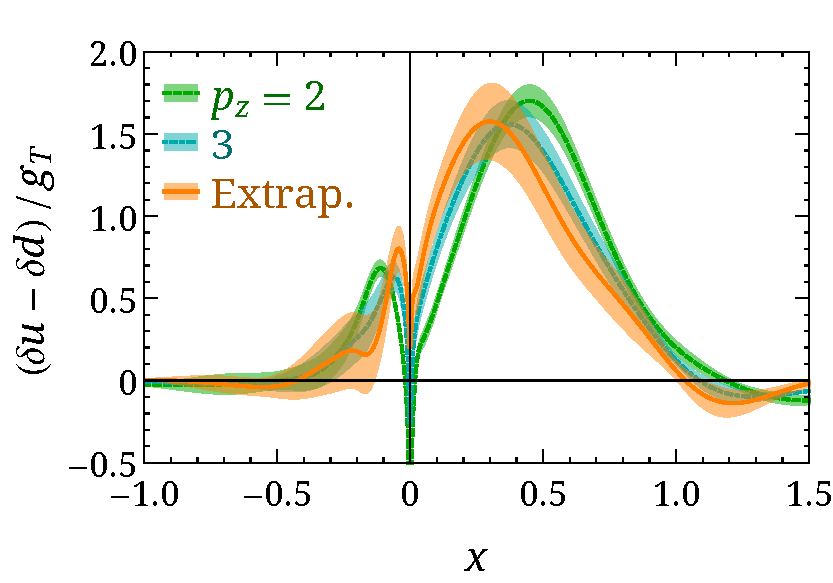
\includegraphics[width=0.32\textwidth]{images/loopscale-transversity-new.pdf}
\vspace*{8pt}
\caption{The momentum-dependence of the nucleon isovector distributions after one-loop and mass correction (i.e. $q_{II}$) for 
 quark density (left), helicity (middle) and transversity (right) as functions of $x$. 
The orange band shows the momentum extrapolation using the higher two momenta.
}
\label{fig:IpM-distribution}
\end{figure}

There are many aspects that need to be improved to get the systematics under control, as indicated at various points in the earlier sections. The operator renormalization also needs to be determined to one-loop level or better in the future calculations. We intend in this work mainly to demonstrate that one can achieve light-cone quantities with reasonable accuracy using currently available computational resources, and it opens the door for many more lattice-QCD calculations on parton physics.
